\documentclass[a4paper]{report}
\usepackage{geometry}
\usepackage{fullpage}
\usepackage{amsmath}

\usepackage{tikz}
\usetikzlibrary{positioning, calc, shapes.geometric, shapes, shapes.arrows, shapes.multipart, arrows.meta, arrows, decorations.markings, external, trees, backgrounds}


\tikzstyle{Arrow} = [
	thick, 
	decoration={
		markings,
		mark=at position 1 with {
			\arrow[thick, -stealth]{latex}
			}
		}, 
	shorten >= 3pt, preaction = {decorate}
	]

\begin{document}

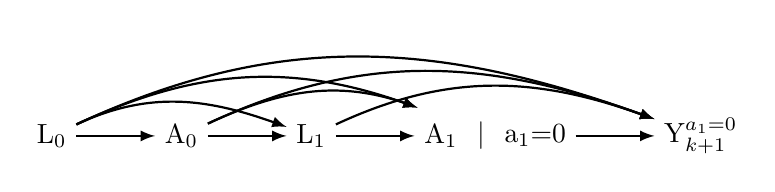
\begin{tikzpicture}[
array/.style={rectangle split, 
	rectangle split parts = 3, 
	rectangle split horizontal, 
    minimum height = 2em
    }
]
 \node (1) {L$_0$};
  \node [right =of 1] (2) {A$_0$}   ;
 \node [right =of 2] (3) {L$_1$};
   \node [array, right =of 3] (4) {
 	{A$_1$}
    \nodepart{two}{$|$} 
    \nodepart{three}{a$_1$=0}
    };
 \node [right =of 4] (5) {Y$_{k+1}^{a_1=0}$};

 \draw[Arrow, thick] (1.east) -- (2.west);
 \draw[Arrow, thick] (1) to [out=25, in=160] (3); 
 \draw[Arrow, thick] (1) to [out=25, in=160] (4); 
 \draw[Arrow, thick] (1) to [out=25, in=160] (5); 
 
 \draw[Arrow, thick] (2.east) -- (3.west);
 \draw[Arrow, thick] (2) to [out=25, in=160] (4);
 \draw[Arrow, thick] (2) to [out=25, in=160] (5);

 \draw[Arrow, thick] (3.east) -- (4.west);
 \draw[Arrow, thick] (3) to [out=25, in=160] (5);

 \draw[Arrow, thick] (4.east) -- (5.west); 
 
\end{tikzpicture}

\end{document}
